\chapter{Nonconvex Problems}
In the last chapter, we treated functionals where we have assumed that the volume density is convex in the third argument, i.e. $A\longmapsto f(x,u,A)$ convex. This, as well as some additional assumptions, ensured that the functional $I(u)=\int_\Omega{f(x,u(x),\nabla u(x))\mathrm{d}x}$ become weakly lower semicontinuous on $W^{1,p}(\Omega;\mathbb{R}^m)$. In general, this convexity-assumption is sufficient but not necessary. In fact, if $\min\{m,d\}=1$, it is also necessary as we have seen in the exercise lessons. Moreover, in some applications convexity in $A$ is a too strong assumption. We will have a look at an application from continuum mechanics (nonlinear elasticity) as a motivating example. In fact, this example is one of the main reasons why the theory we are going to treat in this chapter was developed.\\

Let's consider $\Omega\subset\mathbb{R}^d$ describing a reference configuration of some elastic body and a function $u:\Omega\longrightarrow\mathbb{R}^d$ which describes the deformation of the body in presence of some external forces $F$.

\begin{figure}[ht]
	\centering
	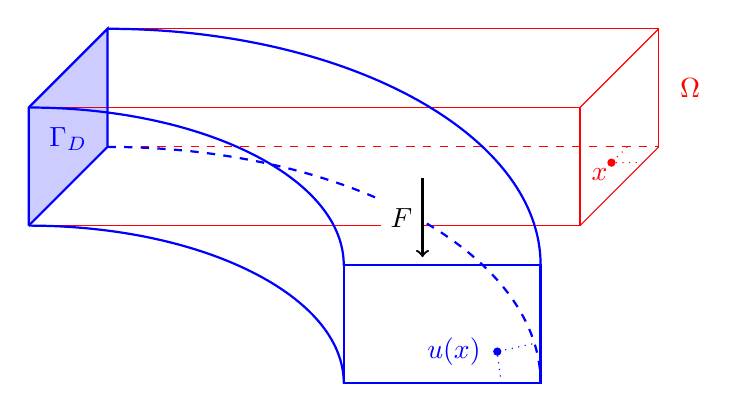
\begin{tikzpicture}
		\draw[red] rectangle (7, 1.5);
		\draw[red] (1, 1) -- (1, 2.5) -- (8, 2.5) -- (8, 1);
		\draw[red, dashed] (1, 1) -- (8, 1);
		\draw[red] (0, 0) -- (1, 1) (7, 0) -- (8, 1) (0, 1.5) -- (1, 2.5) (7, 1.5) -- (8, 2.5);

		\fill[red] (7.4, 0.8) circle (1.5pt);
		\draw[red, dotted] (7.6, 1) -- (7.4, 0.8) -- (7.8, 0.8);

		\draw[thick, blue, fill=blue, fill opacity=0.2] (0, 0) -- (1, 1) -- (1, 2.5) -- (0, 1.5) -- (0, 0);
		\draw[thick, blue] (0, 0) arc (90:0:4 and 2);
		\draw[thick, blue, dashed] (1, 1) arc (90:0:5.5 and 3);
		\draw[thick, blue] (0, 1.5) arc (90:0:4 and 2);
		\draw[thick, blue] (1, 2.5) arc (90:0:5.5 and 3);
		\draw[thick, blue] (4, -2) rectangle (6.5, -0.5);

		\fill[blue] (5.95, -1.6) circle (1.5pt);
		\draw[blue, dotted] (6, -2) -- (5.95, -1.6) -- (6.4, -1.5);

		\draw[thick, ->] (5, 0.6) -- node[left, fill=white] {$F$} (5, -0.4);

		\node[red] at (8.4, 1.75) {$\Omega$};
		\node[red] at (7.25, 0.65) {$x$};
		\node[blue] at (5.4, -1.6) {$u(x)$};
		\node[blue] at (0.5, 1.1) {$\Gamma_D$};
	\end{tikzpicture}
	\caption{Illustration of an elastic deformation with fixed side.}
\end{figure}

The elastic energy of the body is
\[\int_\Omega{f(x,\nabla u(x))\mathrm{d}x},\]
and it is independent of $u$ since constant shifting or rotation should not change the energy. The function $f$ is called ``stored elastic energy density''. The deformation $u$ is the minimizer of
\[I(u)=\int_\Omega{f(x,\nabla u(x))\mathrm{d}x}-\ell(u),\]
where $\ell\in(W^{1,p}(\Omega;\mathbb{R}^d))'$, e.g.
\[\ell(u)=\int_\Omega{F(x)\cdot u(x)\mathrm{d}x}+\int_{\Gamma_N}{G(x)\cdot u(x)\mathrm{d}a}.\]
The first integral could describe gravity and the second some Neumann boundary condition. Physically relevant properties of $f$ are:
\begin{itemize}
	\item[(a)] If we think of a sponge, the energy should increase if we stretch or shrink it. The displacement $u(x)=sx$ describes such an action, and for such $u$ it holds $\nabla u(x)=s\mathrm{Id}$. Thus, we would like to have $f(x,s\cdot\mathrm{Id})>f(x,\mathrm{Id})$ for all $s\ne1$.
	\item[(b)] We also would like to have an invariance property of the form: For all rotations $R\in\SO{d}$ and all $A\in\mathbb{R}^{d\times d}$ it holds $f(RA)=f(A)$.\\

	For example, consider a displacement $u:\Omega\longrightarrow\mathbb{R}^d$ and $\widetilde{u}(x)=Rx+r$, where $Rx$ describes a rotation and $r$ a translation. The gradient of the composition $\widehat{u}=\widetilde{u}\circ u$ is then just $\nabla\widehat{u}=R\nabla u$. The invariance property gives $f(\nabla\widehat{u})=f(\nabla u)$.\\

	So, rigid-body transformation do not change the elastic energy. This is also known as ``objectivity'' (a change of frame of reference is a rigid-body transformation).
\end{itemize}
But there is a problem: There is no convex $f:\mathbb{R}^{d\times d}\longrightarrow\mathbb{R}$ which satisfies the properties (a) and (b) simultaneously. Consider the case $d=2$. Then
\[R=\begin{pmatrix}
	\cos(\vartheta)&-\sin(\vartheta)\\
	\sin(\vartheta)&\cos(\vartheta)
\end{pmatrix}\in\SO{2}.\]
If $f:\mathbb{R}^{2\times 2}\longrightarrow\mathbb{R}$ was convex, then for $A=\frac{1}{2}(R+R^\top)=\cos(\vartheta)\mathrm{Id}$ we would have
\[f(A)=f\left(\frac{1}{2}R+\frac{1}{2}R^\top\right)\leq\frac{1}{2}f(R)+\frac{1}{2}f(R^\top)=f(\mathrm{Id})\]
by property (b). But, if $\cos(\vartheta)<1$, property (a) would give us also $f(A)=f(\cos(\vartheta)\mathrm{Id})>f(\mathrm{Id})$.\\

Likewise one can show for general $d\geq2$ that no such $f$ exists.